\documentclass[../rapport_MVEX01-11-05]{subfiles}
\begin{document}

\subsection{$k$-nearest-neighbour}\label{sec:knn}

\knn eller $k$ närmsta grannar är en klassificeringsmetod som baserat på
prototypobjekt i egenskapsrummet tilldelar en klass observerad punkt i rummet.
Prototypobjekten är en redan klassificerad inlärningsmängd, och vi undrar vilken
av dessa klasser vår observation tillhör.

Klasserna är här olika statiska gester, eller olika grupper i featurerummet. För varje observerad bildruta ska vi alltså undersöka om den hör till någon av de kända klasserna.

Avståndet som används är det euklidiska, dvs
\begin{equation*}
    d = |\vect{x}-\vect{x_0}|^{1/n}
\end{equation*}
där $n$ är dimensionen på egenskapsrummet. Genom en uttömmande sökning i featurerummet letar vi efter de $k$ närmsta grannarna. Om $k$ är större än ett avgörs klasstillhörigheten genom majoritetsomröstning, dvs. den klass med flest nära grannar vinner, se figur \ref{fig:knn-overview}.

\begin{figure}[!htb]
    \begin{center}
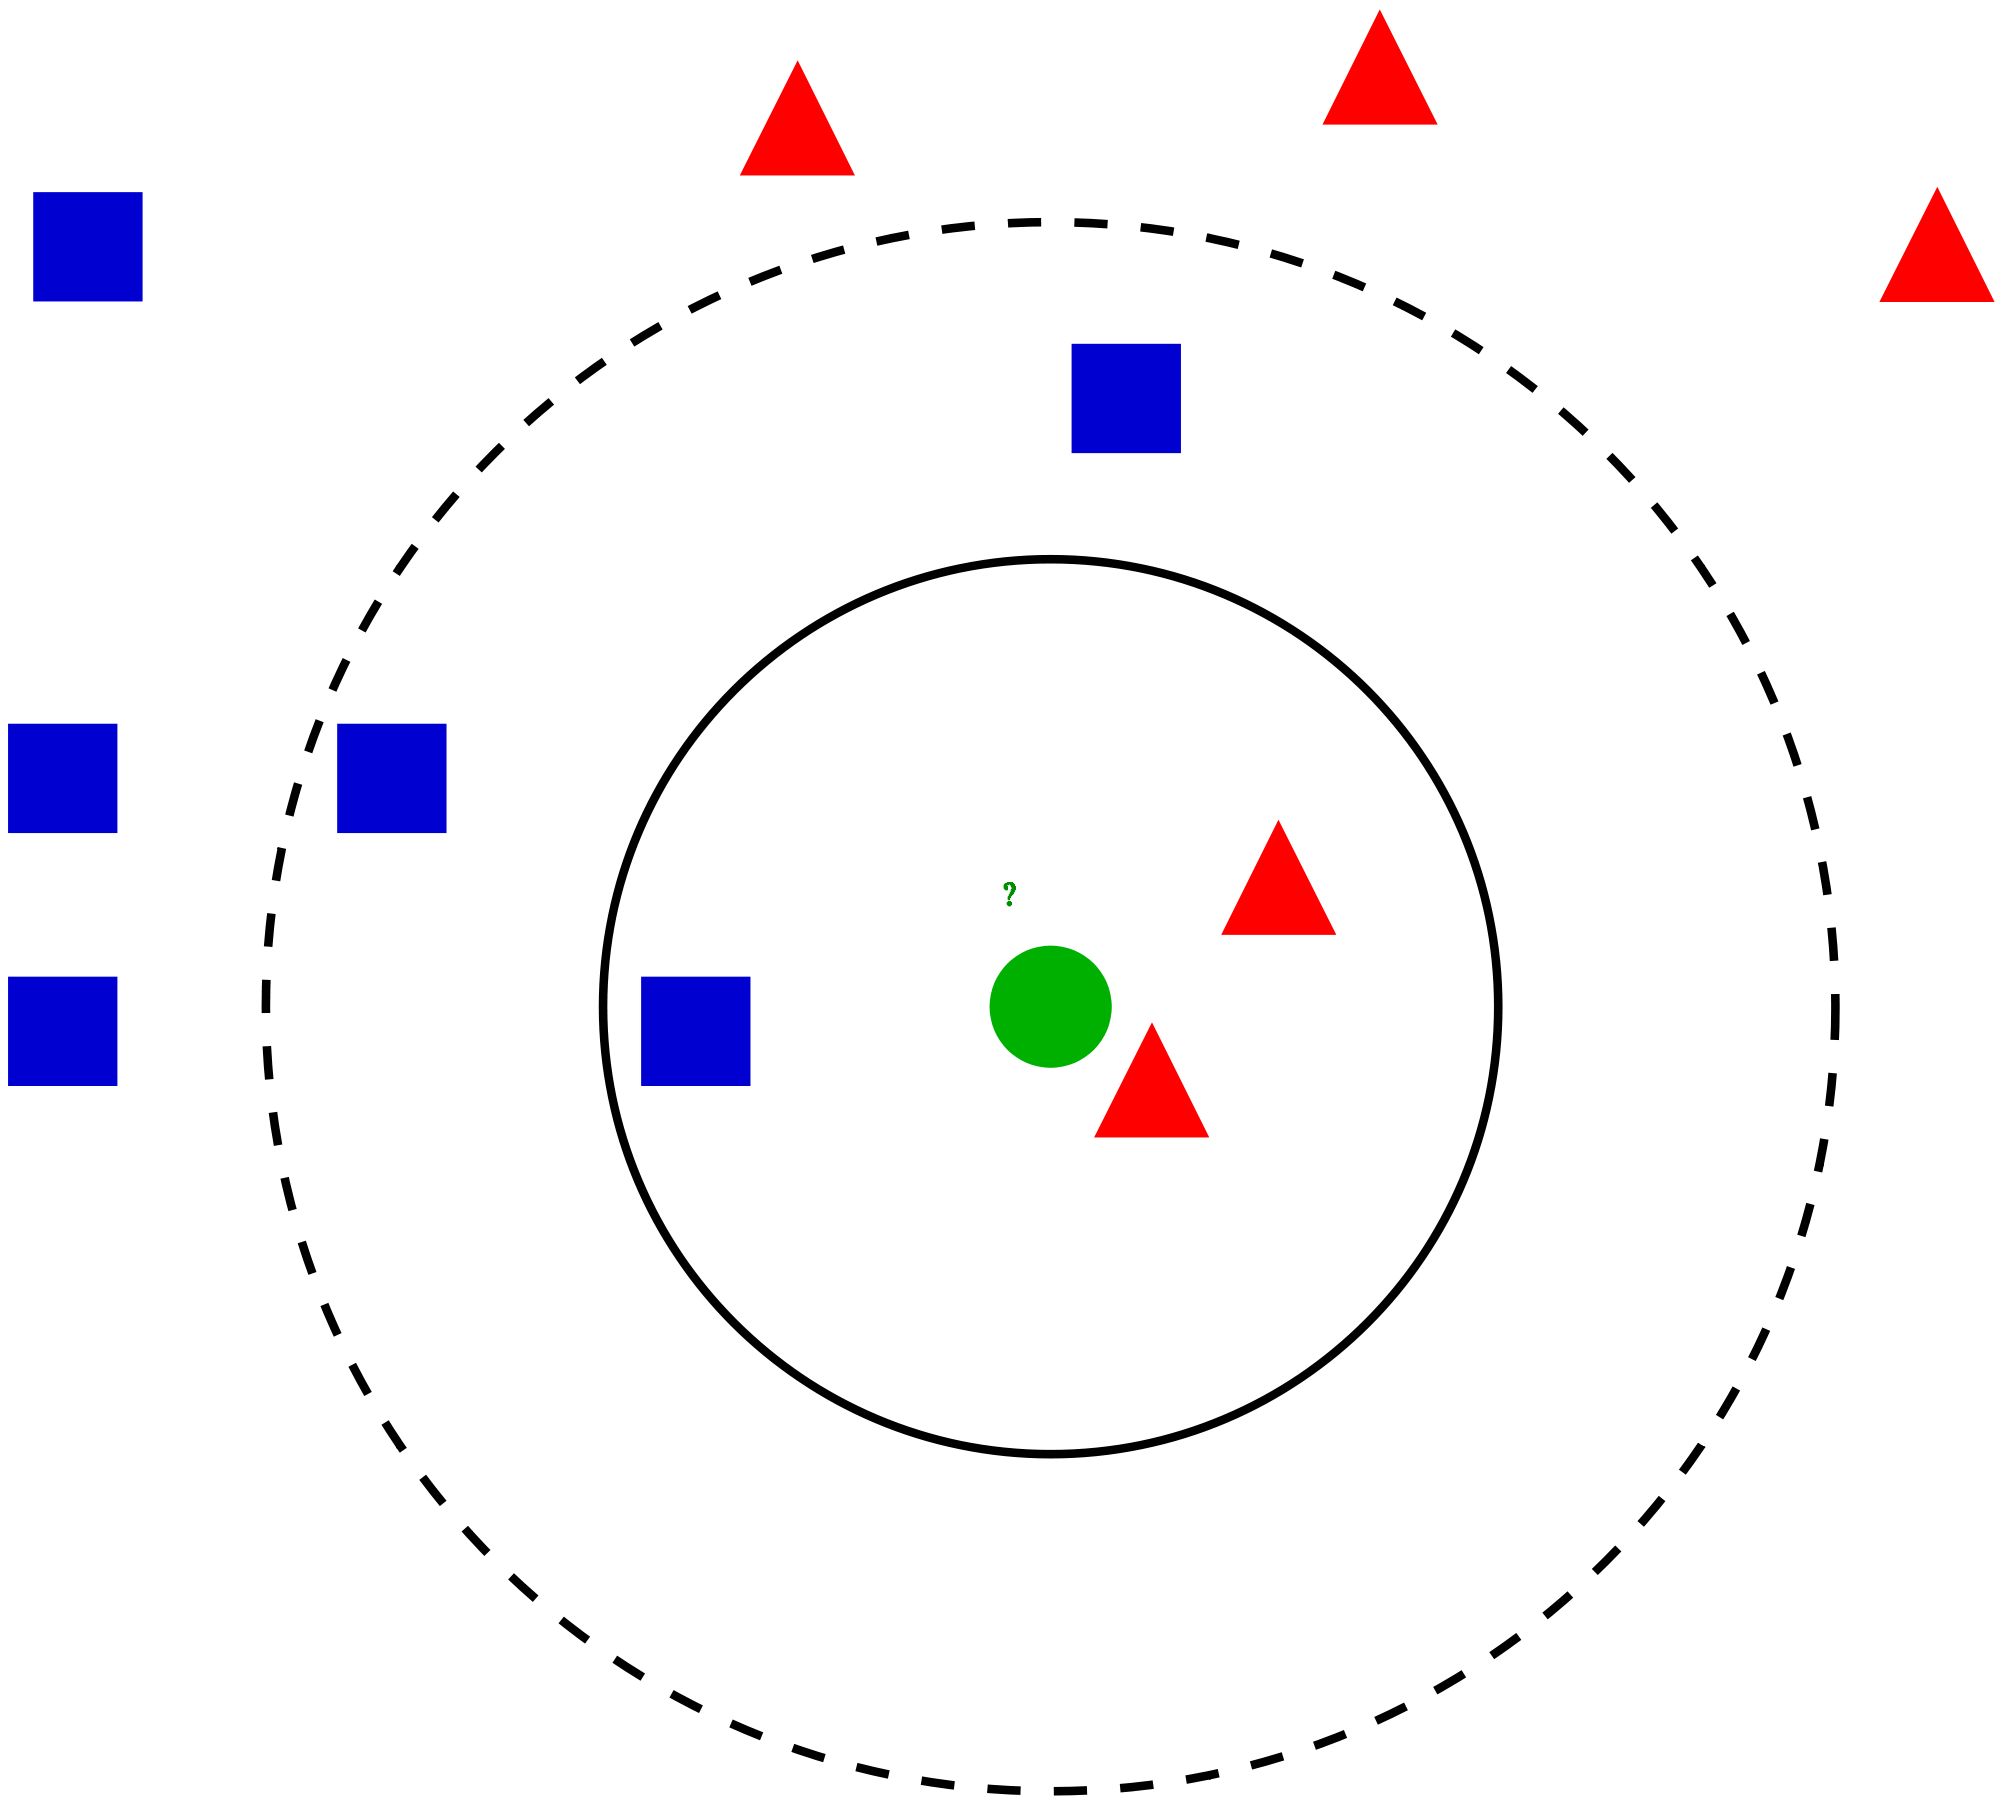
\includegraphics[width=0.75\columnwidth]{bilder/2000px-KnnClassification.jpg}
    \end{center}
    \caption{kNN-klassificering av den runda observationen i mitten i ett rum
    med två klasser, trianglar och kvadrater. Majoritetsomröstning
    med $k=3$ leder till att den runda klassas som triangel, medan $k=5$ leder
    till klassificering som kvadrat.}
    \label{fig:knn-overview}
\end{figure}

För att metoden ska fungera krävs att alla klasser är representerade med lika många prototypobjekt. Annars får vissa klasser större vikt och kommer med högre sannolikhet att väljas.

\notes{referenser?}

%Detta måste givetvis göras en gång per gest, vilket ger oss en kodbok
%per gest; detta eftersom vi har en HMM per gest.
%
%\marginpar{Eller, hur ska vi göra egentligen? En eller flera
% kodböcker? Hur skalar algoritmerna, hur jobbigt blir det? Säger
% någon referens något om detta?}

%FIGUR
%http://en.wikipedia.org/wiki/File:KnnClassification.svg


\end{document}